\documentclass{llncs}

\usepackage{amssymb}
\usepackage{tikz}
\usetikzlibrary{arrows,decorations,positioning,backgrounds,shapes,shapes.multipart,matrix}
\usepackage{pgfplots}
\usepackage{subfigure}
\pgfplotsset{compat=1.9}
\usepgfplotslibrary{groupplots}
\usepackage[boxed,vlined,linesnumbered,noresetcount]{algorithm2e}
\newtheorem{thm}{Theorem}
\newtheorem{lem}{Lemma}
\usepackage{listings}
\usepackage{paralist}
\usepackage{wrapfig}
\usepackage{verbatim}
\usepackage{cite}
\usepackage{multirow}
\lstset{numbers=left}
\usepackage{float}
\usepackage[normalem]{ulem}
\SetAlgorithmName{Alg.}{List of Algorithms}
\SetAlFnt{\small}
\SetKw{KwDownto}{downto}
\setcounter{tocdepth}{3}
\usepackage{graphicx}
\renewcommand\topfraction{0.95}
\renewcommand\bottomfraction{0.95}
\renewcommand\textfraction{0.05} 
\renewcommand\floatpagefraction{0.95}
\renewcommand{\dbltopfraction}{0.95}
\renewcommand{\dblfloatpagefraction}{0.95} 

\usepackage{url}

\SetAlgoSkip{}
\SetKwProg{Fn}{Function}{}{end}
\begin{document}

\mainmatter  % start of an individual contribution

% first the title is needed
\title{Practical Concurrent Unrolled Linked Lists Using Lazy Synchronization}

% a short form should be given in case it is too long for the running head
%%\titlerunning{Lecture Notes in Computer Science: Authors' Instructions}

% the name(s) of the author(s) follow(s) next
%
% NB: Chinese authors should write their first names(s) in front of
% their surnames. This ensures that the names appear correctly in
% the running heads and the author index.
%
\author{Kenneth Platz\and Neeraj Mittal\thanks{This work was supported, in part, by the National Science Foundation (NSF) under grant number CNS-1115733}\and S. Venkatesan}
%
%\authorrunning{Lecture Notes in Computer Science: Authors' Instructions}
% (feature abused for this document to repeat the title also on left hand pages)

% the affiliations are given next; don't give your e-mail address
% unless you accept that it will be published
\institute{The University of Texas at Dallas,\\
Richardson, TX 75080\\
\texttt{\{kplatz, neerajm, venky\}@utdallas.edu}}

%
% NB: a more complex sample for affiliations and the mapping to the
% corresponding authors can be found in the file "llncs.dem"
% (search for the string "\mainmatter" where a contribution starts).
% "llncs.dem" accompanies the document class "llncs.cls".
%

\toctitle{Practical Unrolled Linked Lists Using Lazy Synchronization}
%%\tocauthor{Authors' Instructions}
\maketitle


\begin{abstract}
Linked lists and other list-based sets are one of the most ubiquitous
data structures in computer science.  They are useful in their
own right and are frequently used as building blocks in other
data structures.  A linked list can be ``unrolled'' to combine multiple
keys in each node; this improves storage density and overall performance.
This organization also allows an operation to skip over nodes which cannot 
contain a key of interest.
This paper introduces a new high-performance concurrent unrolled linked list
with  a lazy synchronization strategy that allows
wait-free read operations.  Most write operations under this strategy
can complete by locking a {\em single} node.  
Experiments show up to a 300\% improvement over other concurrent list-based sets.
\keywords{concurrent data structures, lazy synchronization, linked lists}
\end{abstract}


\section{Introduction}

In recent years, processor manufacturers have shifted their 
development focus away from increasing clock speeds and
single-threaded performance.  The rising prevalence of
multi-core and multi-processor systems adds additional import
to the quest for high-performance data structures that permit
concurrent reads and writes while maintaining correct
behavior.

Concurrent data structures can synchronize via several
methods; the most common techniques involve locking.  An
exclusive lock can
be used to control access to some portion of a data structure.
When a thread attempts
to access a portion of a data structure, it must first acquire
one or more locks.  Multiple techniques exist offering varying
degrees of performance.  The performance of a technique depends
upon both the number of locks which must be acquired
during an operation and the {\em granularity} of each lock
(the fraction of the data structure protected by each lock).

Other algorithms use atomic read-modify-write instructions
in lieu of locks.  These instructions, such as compare-and-swap (CAS) or
load-linked/store conditional (LL/SC), can be used to provide lock-free
or wait-free synchronization {\cite{Herlihy:Progress}}. Efficient lock-free and
wait-free algorithms are inherently more complex than lock-based algorithms;
they are harder to design, analyze, implement, and debug. 

The linked list is one of the most ubiquitous data structures in
computer science.  It implements the standard set operations:
{\em insert}, {\em remove}, and {\em lookup}.  A linked list is typically
implemented via a sequence of {\em nodes}, each of which contains a
{\em key}, possibly a {\em data} element, and a pointer to the {\em next}
node in the sequence.  Linked lists are of particular interest because
many other data structures (such as graphs and
hash tables) use linked lists as ``black box'' subroutines
\cite{Cormen:Algorithms}.

Linked lists have been well-studied from a concurrency perspective.
Several efficient lock-based algorithms exist.  The simplest algorithm
consists of a single lock which protects all accesses to the list,
but this does not allow for any true concurrency.  Improvements
have been seen with fine-grained locking, where each node contains
its own lock.  These fine-grained algorithms typically scan the
list for a node of interest and acquire the lock
on that node (and possibly other nodes). Two algorithms that use this technique
include an ``optimistic'' algorithm by Herlihy and Shavit
{\cite{Herlihy:TAOMP}} and a ``lazy'' algorithm by Heller 
{\cite{Heller:LazyList}}.

Linked lists, while extremely useful, do have several disadvantages.  
One major disadvantage to a linked list is that any operation must,
on average, traverse half the nodes in the list.  Each step in this
traversal must dereference that node's next pointer and access
a memory location that may be far removed from the prior node.  This
access pattern makes poor use of the memory hierarchy found in today's
systems.

Several attempts have been made to increase the efficiency of linked
lists by combining multiple keys into a single node.  These ``unrolled'' 
lists, first described by Shao et al \cite{Shao:UnrollingLists}, improve performance
in two ways.  First, unrolling reduces the number of pointers which must be followed
to find an item.  Second, this groups multiple successive elements in sequential
memory locations and better conforms to the principle of
spatial locality {\cite{Demaine:CacheOblivious, Patterson:COD5}}.

More recently Braginsky and Petrank developed a ``chunked'' lock-free linked list
\cite{Braginsky}.  Their algorithm improves the locality of memory accesses
by storing a sequential subset of key/data pairs within a
contiguous block of memory.  As time elapses and elements are inserted
and removed from the list, their algorithm splits full chunks and combines
sparsely populated ones.  An operation can quickly locate
the appropriate chunk, and searches within a chunk exhibit favorable
spatial locality.

\paragraph{Our Contributions:} We present a new lock-based data structure
for an unrolled linked list based upon Heller's lazy synchronization wherein
the majority of operations complete by
locking a {\em single} node.  We allow our data structure to contain up to 
$K$ key/data pairs per node; this improves both the storage density and
locality of reference within a node \cite{Demaine:CacheOblivious}.  Using the algorithms we present,
we can traverse this data structure in $O(n/K + K)$ operations, where
$n$ is the number of key/data pairs stored in the list.  We also sketch a proof
of correctness, using linearizability and deadlock-freedom as our
safety and liveness properties, respectively.

The data structure we present is straightforward to implement and exhibits
excellent throughput.  Our analysis shows that it 
\begin{inparaenum}[(i)]
\item exhibits high degrees of {\em spatial and temporal locality} by accessing
sequential memory locations; 
\item responds extremely well to common {\em compiler optimizations};
and \item increases {\em cache efficiency} by eliminating extraneous pointers.
\end{inparaenum}
In performance testing our implementation
provides up to 300\% higher throughput than the list presented by Braginsky and 
Petrank{\cite{Braginsky}}; the improvement over other concurrent lists is even higher.

\paragraph{Roadmap:} The rest of the paper is as follows.  Section~\ref{Section:Related} describes prior work related to this paper.  Section~\ref{Section:Model} briefly describes our system model.  Section~\ref{Section:Algorithms} describes our data structure, the algorithms to implement standard set operations, and outlines a proof of correctness.  Section~\ref{Section:Experiments} describes our experiments and
analyzes the results and Section~\ref{Section:Optimizations} describes further considerations and optimizations.  Section~\ref{Section:Conclusions} consists of our conclusions and suggestions for further work.

\section{Related Work}\label{Section:Related}
Linked lists have been extensively studied in terms of concurrency;
A number of lock-free and lock-based algorithms
for linked lists exist, including lock-free algorithms by
Valois{\cite{Valois:LFLists}}, Michael{\cite{Michael:LFListSets}}, and 
Harris{\cite{Harris:PragmaticLists}}.
In this paper, we present a lock-based algorithm which permits wait-free reads.

The data structure presented here is modeled after a list by Heller which uses
a ``lazy'' locking strategy\cite{Heller:LazyList}.  This implementation
stores all keys in sorted order; a {\em scan}
identifies the first key greater than or equal to the target key.  The
scan returns a {\em window} of two nodes: a node of interest
and its immediate predecessor.  A {\em lookup} operation returns {\sc true} if
the key of the current node matches the key in question and {\sc false} otherwise.
An {\em insert} or {\em remove} operation obtains a {\em window} from a scan
operation and locks the predecessor and current nodes
(in that order).  The thread must next perform a {\em validate}; another thread may
modify this section of the list before we acquire the locks.  
An {\em insert} then splices a new node into the
list while a {\em remove} removes the node from the list.

Braginsky and Petrank recently developed a ``chunked'' lock-free linked list\cite{Braginsky}
which stores multiple sequential elements within the same memory block.  This chunked list
maintains chunk sizes within a specified minimum and maximum by splitting overfull chunks
and merging underfull neighboring chunks.  A merge or split requires 
``freezing'' the chunk(s) in question to prevent further operations on 
a chunk.  The operation must then {\em stabilize} the chunk to quiesce all pending operations.  
Multiple threads can help with the freeze and stabilize operations.
\section{System Model}\label{Section:Model}
Our data structure implements a list-based set that supports
three operations.  A {\em lookup} operation accepts a {\em key} as an argument and returns either
a {\em data} element indicating success or {\sc nil} indicating failure.  An {\em insert}
operation accepts a {\em key} and {\em data} element as arguments, returning
{\sc true} if the operation successfully inserted the key/data pair or 
{\sc false} to indicate failure (due to the key already existing in the 
list)\footnote{Sets do not permit multiple entries for a given key.  Another option
is to replace the existing data element with the new element.}. 
A {\em remove} operation accepts a {\em key} and returns {\sc true} for success or {\sc false}
if the element was not found.

Our algorithms use exclusive locks for coordination between threads.  
Many locks exist which provide different performance characteristics and
progress guarantees.  We assume a ``black-box'' lock which provides the
guarantees of {\em deadlock-freedom} and {\em mutual exclusion}.  For the sake of brevity, 
we rely on the Resource Acquisition Is Initialization (RAII)\cite{Stroustrup:Design}
idiom when acquiring these locks.  We assume that acquiring a lock involves creating
object with local scope which releases the lock when destroyed. 
In C++11, this is implemented with the \texttt{std::lock\underline{\hspace{5pt}}guard} class.
Other languages have similar constructs, either language-provided or user-specified. 

\section{An Unrolled Linked List Using Lazy Synchronization}\label{Section:Algorithms}

\subsection{Algorithm Overview}
Our unrolled linked list maintains a singly-linked list
of nodes and stores keys in partially sorted order.  Each node contains
\begin{inparaenum}[(i)] 
\item an array of {\em key/data} pairs,
\item a {\em next} pointer to the next node in the list, 
\item a {\em count} of the number of elements in the node, 
\item an exclusive {\em lock},
and \item a {\em marked} flag indicating a node's logical removal. 
\end{inparaenum}
In this data structure {\em lock} protects access to the {\em next} pointer which
allows most operations to complete while holding a single lock. 
We define the parameter $K$ to indicate the maximum number 
of key/data pairs per node and the {\em anchor key} as 
the first key in a node.  We further define parameters {\sc MinFull} and 
{\sc MaxMerge}. {\sc MinFull} is the minimum number of keys before
we attempt to merge nodes; {\sc MaxMerge} is the maximum number of
keys we allow in a merged node.

The data structure keeps track of the {\em head} pointer which
points to the first element in the list.  We maintain two invariants:
\begin{inparaenum}[(i)]
\item the anchor key of each node is strictly less than the anchor key of its successors and 
\item all (non-anchor) keys in a node are strictly greater than their
anchor key.
\end{inparaenum}
We do not impose any ordering among keys within a node;
attempting to keep keys in sorted order would penalize write performance
and complicate wait-free lookups.
The layout of the data structure is depicted in Fig.~\ref{Layout}.

\begin{figure}
\begin{center}
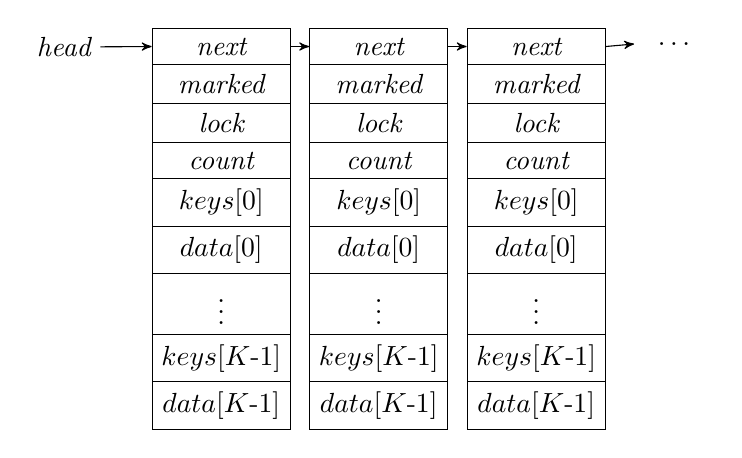
\begin{tikzpicture}[>=stealth']
\node[anchor=north](head)   at (0,0)   {\em head};
\node[draw=black!100,rectangle split,rectangle split allocate boxes=9,
      rectangle split parts=9,anchor=north,
      minimum width=10mm] at (2,0) (next1) 
      {{\em next} \nodepart{two}{\em marked} \nodepart{three}{\em lock}
      \nodepart{four}{\em count} 
      \nodepart{five}{$keys[0]$} \nodepart{six}{$data[0]$}
      \nodepart{seven}{$\vdots$} 
      \nodepart{eight} {$keys[K$-1]} \nodepart{nine}{$data[K$-1]}};
\node[draw=black!100,rectangle split,rectangle split allocate boxes=9,
      rectangle split parts=9,anchor=north,
      minimum width=10mm] at (4,0) (next2) 
      {{\em next} \nodepart{two}{\em marked} \nodepart{three}{\em lock}
      \nodepart{four}{\em count} 
      \nodepart{five}{$keys[0]$} \nodepart{six}{$data[0]$}
      \nodepart{seven}{$\vdots$} 
      \nodepart{eight} {$keys[K$-1]} \nodepart{nine}{$data[K$-1]}};
\node[draw=black!100,rectangle split,rectangle split allocate boxes=9,
      rectangle split parts=9,anchor=north,
      minimum width=10mm] at (6,0) (next3) 
      {{\em next} \nodepart{two}{\em marked} \nodepart{three}{\em lock}
      \nodepart{four}{\em count} 
      \nodepart{five}{$keys[0]$} \nodepart{six}{$data[0]$}
      \nodepart{seven}{$\vdots$} 
      \nodepart{eight} {$keys[K$-1]} \nodepart{nine}{$data[K$-1]}};
\node[minimum height=4mm,anchor=north,minimum width=10mm](dots) at (7.75,0) {$\dots$};
\draw [->] (head) -- (next1.text west);
\draw [->] (next1.text east) -- (next2.text west);
\draw [->] (next2.text east) -- (next3.text west);
\draw [->] (next3.text east) -- (dots.west);

\end{tikzpicture}
\end{center}
\caption{Layout of the unrolled linked list}
\label{Layout}
\end{figure}

We define two sentinel values of $-\infty$ and $+\infty$.  We
initialize the list with three sentinel nodes with anchor keys of
$-\infty$, $-\infty$, and $+\infty$.  The sentinel value
of $\top$ indicates a key slot that is unused.

Each operation scans the list to find the appropriate node upon which to operate and
returns that node and its predecessor.
An insert replaces a sentinel
key with our new key/data pair and returns {\sc true} if successful or
{\sc false} if the element is already in the list. 
A remove replaces a key with a sentinel key,
returning  {\sc true} for success or {\sc false} for
failure (i.e. the element was not found in the list). 
A lookup returns either the {\em data} element associated with
the key or {\sc nil} if the key is not in the list.

\subsection{Algorithm Detail}

The first step in any operation on the list involves a {\em scan} (Alg.~{\ref{Algorithm:Scan}}).
We maintain three pointers during this scan, {\em prev}, {\em curr}, and {\em succ}.
We scan through the list until the {\em succ} contains an anchor key
greater than our key of interest.  Once {\em succ} meets this criteria,
{\em scan} returns the pair ({\em prev}, {\em curr}).

\begin{algorithm}
\DontPrintSemicolon
\Fn{scan($item$) : (node,node)}{
    $prev \leftarrow head$ \;
    $curr \leftarrow prev.next$ \;
    $succ \leftarrow curr.next$ \;
    \While{ succ.key $>$ item } {
        $prev \leftarrow curr$ \;
        $curr \leftarrow succ$ \;
        $succ \leftarrow succ.next$ \;
    }
    \Return ($prev$,$curr$)\;
}
\caption{Scan}
\label{Algorithm:Scan}
\end{algorithm}

The {\em lookup} function starts with a {\em scan} of the list (Alg.~{\ref{Algorithm:Lookup}).  
Once we have our {\em curr} node, we 
perform a single pass through its keys looking for {\em item}.  At each slot, we read the key/data
pair {\em atomically} (line~\ref{Lookup:AtomicRead}).  We can either select key and data elements 
that collectively fit within a machine word or 
use atomic snapshots~\cite{Afek:Atomic,Anderson:Composite}. 
All of our tested implementations use the former technique\footnote{Specifically we store a 32-bit key and data element 
in a 64-bit word.}~\cite{Braginsky}.
If we encounter {\em key} during our scan, we return the associated
{\em data} element. If we reach the end of the keys without finding {\em item}, 
it may still be present; a concurrent {\em remove} operation 
may relocate {\em item} to the anchor key of  a node.  
In this case, we must re-read the anchor key/data pair.  If {\em item} is present, we return 
its associated {\em data} element; otherwise, we return {\sc nil}.

\begin{algorithm}
\DontPrintSemicolon
\Fn{lookup(item) : Data} {
    $(prev,curr) \leftarrow scan(item)$ \;
    \For{$i \leftarrow 0$ \KwTo $K-1$} { \label{Lookup:Loopbegin}
        $(key, data) \leftarrow (curr.keys[i],curr.data[i])$ \label{Lookup:AtomicRead} \;
        \lIf {key = item} { \Return $data$ \label{Lookup:Loopend} }
    } 
    $(key,data) \leftarrow (curr.keys[0],curr.data[0])$ \;
    \lIf {key = item} { \Return $data$  }
    \Return {\sc nil} \label{LP:Lookup3} \;
}
\caption{Lookup}
\label{Algorithm:Lookup}
\end{algorithm}


Our {\em insert} and {\em remove} functions depend upon a {\em validate} function
(Alg.~{\ref{Algorithm:Validate}}) similar to Heller's{\cite{Heller:LazyList}}. 
We must perform this validation because another thread may still manipulate {\em prev}
or {\em curr} until we acquire the lock on {\em prev}.
We validate by checking that neither {\em prev} nor {\em curr} are marked for removal,
{\em prev.next} still points to {\em curr}, and our target key is not less than 
{\em curr's} anchor key\footnote{A concurrent removal of {\em curr}'s anchor key may
result in this violation.}.
\begin{algorithm*}
\DontPrintSemicolon
\Fn{validate(prev, curr, item) : boolean}{
    \Return $\neg prev.marked\; \wedge\; \neg curr.marked$
    $\wedge\; prev.next = curr\; \wedge\; curr.keys[0] \leq item$ \;
}
\caption{Validate}
\label{Algorithm:Validate}
\end{algorithm*}

The {\em insert} operation (Alg.~{\ref{Algorithm:Insert}}),
performs a {\em scan} to locate an appropriate insertion point, locks
{\em prev}, performs a {\em validate}.  If the validation fails, the operation must return to the head of the list and scan again.
Once a validation succeeds, it checks {\em curr} for three conditions.  If 
{\em curr} already contains {\em item} it leaves the node unchanged
and returns {\sc false}.  If there is at least one empty slot in {\em curr}
(denoted by the sentinel $\top$) it atomically replaces the sentinel key and its 
associated data element with the new key/data pair, increments {\em count}, and returns {\sc true}.   
If there are no available slots, we must split the node.
\begin{algorithm}
\DontPrintSemicolon
\Fn{insert(key,data) : boolean}{
    \While{$true$}{
        ($prev$,$curr$) $\leftarrow$ scan($item$)\;
        $prev$.lock() \;
        \If {$\neg$validate($prev$,$curr$,$item$)} {
            {\bf continue} \tcc*[f]{Return to head and re-scan}
        }
        \lIf {$curr.\mathrm{contains}(item)$} { \label{Insert:Contains}
            \Return {\sc false} 
        }
        $slot \leftarrow$ first location of $\top$ in $curr$ \label{Insert:FindFirst} \;
        \eIf {$slot\mathrm{~is~defined}$} {
            ($curr.\mathrm{keys}[slot], curr.\mathrm{data}[slot])
            \leftarrow (key, data)$ \label{LP:Insert} \;
            $curr.count \leftarrow curr.count + 1$ 
        }  {
            $curr$.lock() \;
            $(new1, new2) \leftarrow$ split($curr$) \;
            \eIf {$key < new2\mathrm{'s~anchor~key}$} {
                $(new1.keys\lceil K/2 \rceil,new1.data\lceil K/2\rceil) \leftarrow (key,data)$ \label{LP:Split1} \;
                $new1.count \leftarrow new1.count + 1$
            } {
                $(new2.keys\lfloor K/2\rfloor,new2.data\lfloor K/2\rfloor) \leftarrow (key,data)$ \label{LP:Split2} \;
                $new2.count \leftarrow new2.count + 1$
            }
            $curr.marked \leftarrow$ {\sc true} \;
            $prev.next \leftarrow new1$ \;
        }        
        \Return {\sc true} \;
    }
}
\caption{Insert}
\label{Algorithm:Insert}
\end{algorithm}
To split a node (Alg.~{\ref{Algorithm:Split}}), we first lock {\em curr}.  
This will not require another validation since no other thread can modify {\em prev.next}. 
Next we allocate two new nodes, {\em new1} and
{\em new2}.  We copy all of the key/data pairs from {\em curr} to {\em new1}, sort 
them\footnote{While there is a $O(n)$ algorithm
to determine the median and partition a set of values, in real-world situations, an efficient
sorting algorithm is faster \cite{Cormen:Algorithms}.}, and then copy the upper half to {\em new2}.  Finally, we replace the upper half
of {\em new1}'s keys with $\top$. 
\begin{algorithm}
\DontPrintSemicolon
\Fn{split(node) : (Node, Node)}{
    Allocate two new nodes, $new1$ and $new2$ \;
    Copy all key/data pairs from $node$ to $new1$ \;
    Sort all key/data pairs in $new1$ ascending by key \;
    Copy the upper $\lfloor K/2 \rfloor$ key/data pairs from $new1$ to $new2$ \;
    Replace the upper $\lfloor K/2 \rfloor$ keys in $new1$ with $\top$ \;
    $new1.next \leftarrow new2$ \;
    $new2.next \leftarrow node.next$ \;
    $new1.count \leftarrow \lceil K/2 \rceil, new2.count \leftarrow \lfloor K/2 \rfloor$ \;
    \Return ($new1$, $new2$) \;
}
\caption{Split}
\label{Algorithm:Split}
\end{algorithm}

\begin{algorithm}
\DontPrintSemicolon
\Fn{remove(item) : boolean} {
    \While{true}{
        $(prev, curr) \leftarrow scan(item)$ \;
        $prev.lock()$ \;
        \If {$\neg$validate($prev$, $curr$,$item$)} {
            \bf{continue} \;
        }
        $slot = curr$.contains($item)$  \label{Remove:Contains} \;
        \If { $slot\mathrm{~is~not~defined}$ }{
            \Return {\sc false} \;
        }
        \eIf { slot = 0 } {
            $min \leftarrow $ location of next smallest key in $curr$ \label{Remove:NextSmallest} \;
            $(curr.keys[0],curr.data[0]) \leftarrow (curr.keys[min],curr.data[min]$  \label{LP:RemoveAnchor} \;
            $curr.keys[min] \leftarrow \top$ \;
        } {
            $curr.keys[slot] \leftarrow \top$ \; \label{LP:Remove}
        }
        $curr.count \leftarrow curr.count - 1$ \;
        
        
        \If {$curr.count < $\sc{MinFull}} {
            $curr$.lock() \;
            $succ \leftarrow curr.next$ \;
            
            \If {$succ.keys[0] = +\infty$ } { \label{MergeTail}
                \Return {\sc true} \;
            }
            \If {$curr.count = 0$} { \label{EmptyNode}
                $curr.marked \leftarrow$ {\sc true}\;
                $prev.next \leftarrow succ$ \;
                \Return {\sc true} \;
            }


            $succ$.lock() \;
            \eIf {$curr.count + succ.count <$ {\sc MaxMerge} }{
                $merge( curr, succ )$ \;
            } {
                $(new1, new2) \leftarrow rebalance( curr, succ )$ \;
                $prev.next \leftarrow new1$ \;
            }
        }
        \Return {\sc true} \;
    }
}
\caption{Remove}
\label{Algorithm:Remove}
\end{algorithm}


Removing an element operates in a similar manner (Alg.~{\ref{Algorithm:Remove}}).  
We perform a {\em scan} to locate the ({\em prev}, {\em curr}) pair, lock  
{\em prev}, and {\em validate}.
If this succeeds, we attempt to locate {\em item}
in {\em curr.keys}.  If it is not present, we return {\sc false}.  If {\em item} is
present but not the anchor key, we replace {\em item} with the sentinel $\top$.
If {\em item} is the anchor key, we locate $min$, the location of our next smallest key.  We then
replace the anchor key/data pair with the $min$ key/data pair and
replace the $min$ key with $\top$.
At this time, we also decrement
the node's $count$.  If our node now has fewer than {\sc MinFull} keys, some
additional checking is required. Specifically, we neither merge with the tail (line~\ref{MergeTail})
nor an empty node (line~\ref{EmptyNode})\footnote{This can happen if {\em succ} is the tail.}.   Otherwise,
we either merge with our successor node (Alg.~\ref{Algorithm:Merge}) 
or create two new nodes and partition the key/data pairs equally among them (Alg.~\ref{Algorithm:Rebalance}).


\begin{algorithm}
\DontPrintSemicolon
\Fn{merge(curr, succ)} {
    Copy valid key/data pairs from $succ$ to $curr$ \;
    $succ.marked \leftarrow $ {\sc true} \;
    $curr.next \leftarrow succ.next$ \;
}
\caption{Merge}
\label{Algorithm:Merge}
\end{algorithm}
\begin{algorithm}
\DontPrintSemicolon
\Fn{rebalance(curr, succ) : (Node, Node)} {
    Create two new nodes $new1$ and $new2$ \;
    Copy valid key/data pairs from $curr$ and $succ$ to $new1$ \;
    $newcount \leftarrow curr.count + succ.count$ \;
    Sort all key/data pairs in $new1$ by ascending key value \;
    Copy the upper $\lfloor newcount/2 \rfloor$ key/data pairs from $new1$ to $new2$ \;
    Replace the upper $\lfloor newcount/2 \rfloor$ keys in $new1$ with $\top$ \;
    $new1.count \leftarrow \lceil newcount/2 \rceil, new2.count \leftarrow
        \lfloor newcount/2 \rfloor$ \;
    $new2.next \leftarrow succ.next$, $new1.next \leftarrow new2$ \;
    $curr.marked \leftarrow $ {\sc true} \;
    $succ.marked \leftarrow $ {\sc true} \;
    \Return ($new1, new2$) \;
}
\caption{Rebalance}
\label{Algorithm:Rebalance}
\end{algorithm}

\subsubsection{Optimization}
We can further modify the above algorithms to keep all valid keys at the head of the node; this
requires minor changes to {\em remove}.  
Instead of replacing the affected key with $\top$, we would replace that key with the 
last valid key in the node and replace the last valid key with $\top$ (this is symmetric to
removing the anchor key).  This effectively can cause a valid key to move forward within a node;
therefore, a {\em lookup} would need to scan from right-to-left to correctly identify
whether the key is present.

\subsection{Correctness Proof}
Here we sketch a proof that our algorithm is correct; we provide more rigorous proof in the accompanying technical report~\cite{Platz:Unrolled}. In our proof, we use deadlock-freedom as 
the liveness property and linearizability as the safety property.  We assume that garbage nodes are never reclaimed (all memory accesses are safe).  We also assume that our key space is finite; any traversal of the list will terminate.  We will make use of the following terms: a {\em write} operation shall consist of an insert or
a remove, an {\em active} node is a node currently reachable from the head of the list,
and a {\em passive} node is a node that is no longer active.  We similarly
define {\em lookup-hit} and {\em lookup-miss} operations.  We can further treat
failed {\em insert} operations as lookup-hits, and failed {\em remove} operations
can be treated as lookup-misses. 

At any moment in time, one or more threads may hold locks on nodes.  We can
order these threads in head-to-tail order according to the lock(s) they hold.  
Since our key space is finite, our list is of finite length; therefore,
one thread will hold the rightmost lock.  Since a thread always acquires locks from
head-to-tail, this thread will always be able to progress.

We can also define a linearization point for every operation.
\begin{itemize}
\item A successful {\em insert} operation either linearizes to when the key/data is written or
(for a split operation) when the $prev.next$ pointer is updated.
\item A successful {\em remove} operation can linearize to the point where $\top$ is written
\item Any {\em lookup} operation which operates on a {\em passive} node can be linearized to
the point at which the node becomes passive.
\item A {\em lookup-hit} operating on an {\em active} node can be linearized at the point
it reads the key/data pair.
\item A {\em lookup-miss} operating on an {\em active} node has two subcases.  If the
key is not present when the thread starts scanning, we can linearize to the instant the
scan begins.  If the key is present at that point, a successful {\em remove} operation must
have removed it.  We can therefore linearize the {\em lookup-miss} immediately to immediately follow the point of the {\em remove}.
\end{itemize}

\section{Experimental Evaluation}\label{Section:Experiments}
\subsection{Experiment Setup}
We completed our experiments on a 2-processor AMD Opteron 6180SE system
with a clock speed of 2.5GHz, 24 total execution cores, and 64GB of memory
running Linux (kernel 2.6.43).  All of our evaluation code was written in
C++ and compiled using gcc-4.8.3 using the same set of 
optimizations (-O3 -funroll-loops -march=native).   
We evaluated the following list implementations:
\begin{enumerate}
\item{\bf Lazy:} The lazy linked list by Heller{\cite{Heller:LazyList}}.
\item{\bf LockFree:} A lock-free linked list by 
Harris\cite{Harris:PragmaticLists} and Michael{\cite{Michael:LFListSets, michael:Hazard}}.
\item{\bf Chunked:} The chunked linked list by Braginsky and 
Petrank{\cite{Braginsky}}\footnote{Source code was obtained 
with permission from Braginsky and Petrank.}.
\item{\bf Unrolled:} The unrolled linked list described in this paper.
\end{enumerate}

Each implementation used hazard pointers for garbage collection.  For our initial
experiments we tested node sizes ranging from 8 to 512 keys per node,  key 
ranges from 1,024 to 1 million, thread counts ranging from 1 to 48, and multiple
workload mixes.  Based on our initial observations, we feel the following parameters
accurately represent the performance of our and other list 
implementations\footnote{Additional experimental data is available in the
companion technical report \cite{Platz:Unrolled}.}:

\begin{enumerate}
\item{\bf Node Size:} For the chunked and unrolled lists, 
we evaluated the performance with $K$ of 8 and 64 keys per node, {\sc MinFull}
of $K$/4 and {\sc MaxMerge} of $3K$/4.
\item{\bf Workload Distribution:} We evaluated performance against three
representative workloads:
{\em write-dominant} with no lookups, 50\% inserts, 50\% removes;
{\em balanced} with 70\% lookups, 20\% inserts, 10\% removes; 
and {\em read-biased} with 90\% lookups, 9\% inserts, 1\% removes.

\item{\bf Degree of Concurrency:} We evaluated the performance with 1, 2, 4,
8, 12, 16, 20, and 24 threads.
\item{\bf Key Range:} Keys were allowed to range from 0 to 5,000 (inclusive)
\end{enumerate}

Each experiment was conducted by initially creating a list with 2,500 entries.  
We then spawned the specified number of threads and ran them concurrently.
Each thread executed as many operations as possible using
the specified mix of operations, and we recorded the total number of operations.
Each experiment was repeated until we achieved a 95\% confidence interval
less than 10\% of the mean.
All results are reported in operations per microsecond.

\tikzstyle{every axis legend}+=[font=\tiny,legend pos=north west]
%\pgfplotsset{every axis legend/.append style
\tikzstyle{every axis ylabel style}+=[font=\tiny]
\tikzstyle{every mark style}+=[solid]
\begin{figure}
\centering
\begin{tikzpicture}


\begin{groupplot}[
    legend columns=3,
    group style={group size=2 by 3,ylabels at=edge left,xlabels at=edge bottom,
                 vertical sep=1.5cm},
    ylabel={Ops per $\mu$sec},
    ylabel style={text height=0.02\textwidth,inner ysep=0pt},
    xlabel style={align=center},
    xlabel={Threads},
    height=0.475\linewidth,width=0.475\linewidth,/tikz/font=\small,
    title style={align=center},
     y filter/.code={\pgfmathparse{#1/10^6}\pgfmathresult}]
    \nextgroupplot[title={$K=8$\\0/50/50 workload}]
    \addplot [color=black!100,mark=star] 
        table [x={threads}, y={lazy}] 
        {data/data_write.txt}; \label{plots:Lazy}
    \addplot [color=black!75,mark=x] 
        table [x={threads}, y={lf}]
        {data/data_write.txt}; \label{plots:LockFree}
    \addplot[color=black!75,mark=square] 
        table [x={threads}, y={chunked}]
        {data/data_write.txt}; \label{plots:Chunked}
    \addplot[mark=*,densely dotted]
        table [x={threads}, y={unrolled}]
        {data/data_write.txt}; \label{plots:Unrolled}
    \coordinate (top) at (rel axis cs:0,1);
    \nextgroupplot[title={$K=64$\\0/50/50 workload}]  
    \addplot [color=black!75,mark=x]
        table [x={threads}, y={lf}]
        {data/data_write.txt};% \label{plots:LockFree}
    \addplot[color=black!75,mark=square]
        table [x={threads}, y={chunked64}]
        {data/data_write.txt}; %\label{plots:Chunked64}
    \addplot[mark=*,densely dotted] 
        table [x={threads}, y={unrolled64}]
        {data/data_write.txt}; % \label{plots:Unrolled64}
    \nextgroupplot[title=70/20/10 workload] % 
    \addplot [color=black!100,mark=star]
        table [x={threads}, y={lazy}]
        {data/data_balanced.txt};  % Lazy
    \addplot [color=black!75,mark=x] 
        table [x={threads}, y={lf}]
        {data/data_balanced.txt}; % LockFree
    \addplot[color=black!75,mark=square] 
        table [x={threads}, y={chunked}]
        {data/data_balanced.txt}; % \label{plots:Chunked8}
    \addplot[mark=*,densely dotted] 
        table [x={threads}, y={unrolled}]
        {data/data_balanced.txt}; % \label{plots:Unrolled8}
    \nextgroupplot[title=70/20/10 workload]
    \addplot [color=black!75,mark=x] 
        table [x={threads}, y={lf}]
        {data/data_balanced.txt};% LockFree
    \addplot[color=black!75,mark=square] 
        table [x={threads}, y={chunked64}]
        {data/data_balanced.txt};% \label{plots:Chunked500}
    \addplot[mark=*,densely dotted] 
        table [x={threads}, y={unrolled64}]
        {data/data_balanced.txt};% \label{plots:Unrolled500}
    \nextgroupplot[title=90/9/1 workload] % 
    \addplot [color=black!100,mark=star] 
        table [x={threads}, y={lazy}]
        {data/data_read.txt}; % Lazy
    \addplot [color=black!75,mark=x] 
        table [x={threads}, y={lf}]
        {data/data_read.txt}; % LockFree
    \addplot[color=black!75,mark=square] 
        table [x={threads}, y={chunked}]
        {data/data_read.txt}; % \label{plots:Chunked8}
    \addplot[mark=*,densely dotted] 
        table [x={threads}, y={unrolled}]
        {data/data_read.txt}; % \label{plots:Unrolled8}
    \nextgroupplot[title=90/9/1 workload]
    \addplot [color=black!75,mark=x] 
        table [x={threads}, y={lf}]
        {data/data_read.txt}; % LockFree
    \addplot[color=black!75,mark=square] 
        table [x={threads}, y={chunked64}]
        {data/data_read.txt};% \label{plots:Chunked500}
    \addplot[mark=*,densely dotted] 
        table [x={threads}, y={unrolled64}]
        {data/data_read.txt};% \label{plots:Unrolled500}
    \coordinate (bot) at (rel axis cs:1,0);
    
\end{groupplot}
  \path (top|-current bounding box.south)--
        coordinate(legendpos)
        (bot|-current bounding box.south);
        
  \matrix[
      matrix of nodes,
      anchor=north,
      draw,
      inner sep=0.2em,
    ]at([yshift=-1ex]legendpos)
    { \ref{plots:Lazy}& Lazy&[5pt]
      \ref{plots:LockFree}& LockFree&[5pt]\\
      \ref{plots:Chunked}& Chunked&[5pt]
      \ref{plots:Unrolled}& Unrolled&[5pt]\\ };        
\end{tikzpicture}
\caption{Experimental Results}
\label{Figure:Performance}
\end{figure}
\subsection{Experimental Results}
Fig.~\ref{Figure:Performance} depicts the results of our experiments.  The graphs on the
left depict results for 8 keys per node while those on the right show 64 keys per 
node.  From top to bottom we display results for the 0/50/50, 70/20/10, and 90/9/1 workloads,
respectively.  These results show that the relative performance of each algorithm remains
consistent for every workload and thread count.  Specifically, we can rank them fastest to
slowest: our unrolled algorithm, Braginsky and Petrank's chunked algorithm, Harris and Michael's
lock-free algorithm, and Heller's lazy algorithm.  The relative throughput at 24 threads is shown
in Table~\ref{Figure:RelativePerf}.
\begin{table}
\setlength{\tabcolsep}{6pt}
\centering
\begin{tabular}{| c | c | c | c | c | c | c |}
\cline{4-7}
\multicolumn{3}{c}{}&\multicolumn{2}{|c|}{$K = 8$}&\multicolumn{2}{|c|}{$K = 64$}\\
\hline
Workload&Lazy&Lock-Free&Chunked&Unrolled&Chunked&Unrolled\\
\hline
0/50/50&100 & 112 & 143 & 291 & 311 & 1012\\
\hline
70/20/10& 100 & 108 & 177 & 435 & 665 & 1745\\
\hline
90/9/1& 100 & 114 & 160 & 406 & 1086 & 2211\\
\hline
\end{tabular}
\caption{Relative throughput at 24 threads with respect to the Lazy algorithm}
\label{Figure:RelativePerf}
\end{table}

Intuitively we can divide the four algorithms into two groups.  The lazy and lock-free lists
operate as a single phase; each step along the list visits each entry in turn.  The
chunked list and unrolled list take a two phase approach.  The first phase skips over 
multiple entries while seeking the correct node, and the second phase scans sequential entries
in that node.

When we consider the performance differential between our data structure
and the chunked list, we should consider the following points:
\begin{enumerate}
\item A lookup in the chunked list (once the node has been identified)
involves repeatedly dereferencing a pointer and accessing a different area of the chunk.  Our
list scans sequentially through an array.  This provides the added benefit of
{\em spatial locality}\cite{Hennessy:CArch5}.  When we access a key/data pair, it is likely on the same
cache line as the last-accessed pair.\footnote{On the AMD architecture we tested, a key/data
pair consumes 8 bytes, and the cache line stores 64 bytes.  This allows 8 key/data pairs to share a
cache line.} Compilers can also aggressively optimize array scans
using techniques such as loop unrolling, cache prefetching and software
pipelining\cite{Aho:Compilers}.  A compiler can (in some cases) also use
vector instructions to perform multiple comparisons concurrently.
\item In order to perform a split, merge, or rebalance, the chunked list must first freeze
and stabilize the affected node(s).  Freezing requires visiting each entry and setting a freeze bit (using CAS)
while stabilizing involves traversing the chunk and removing any partially-deleted nodes.
Our list only requires two calls to the {\em copy}
library routine and one call to the {\em sort} routine to perform either operation.
These library routines are typically aggressively optimized for performance. 
\end{enumerate}


In order to measure the effect of compiler optimizations on our list and the chunked list, we 
disabled all optimizations and recompiled.  We then re-ran our experiments using the balanced  workload with 8 and 64 keys per node.  We then compared the performance and calculated the speedup percentage for each degree of concurrency (Figs.~\ref{Figure:Optimized1}~and~\ref{Figure:Optimized2}).
\begin{figure}
\centering
\begin{tikzpicture}
\begin{groupplot}[
    legend columns=3,
    group style={group size=2 by 1,ylabels at=edge left},
    ylabel={Ops per $\mu$sec},
    ylabel style={text height=0.02\textwidth,inner ysep=0pt},
    xlabel={Threads},
    title style={align=center},
         y filter/.code={\pgfmathparse{#1/10^6}\pgfmathresult},
    height=0.475\linewidth,width=0.475\linewidth,/tikz/font=\small]
    
    \nextgroupplot[title={$K=8$}]
    \addplot[color=black!50,mark=triangle]  
        table [x={threads}, y={chunked0}]
        {data/optimized.txt}; \label{plots:ChunkedNo}
    \addplot[mark=square,color=black!100] 
        table [x={threads}, y={chunked3}]
        {data/optimized.txt}; \label{plots:ChunkedYes}
    \addplot[color=black!50,mark=star]  
        table [x={threads}, y={unrolled0}]
        {data/optimized.txt}; \label{plots:UnrolledNo}
    \addplot[mark=o,color=black!100] 
        table [x={threads}, y={unrolled3}]
        {data/optimized.txt}; \label{plots:UnrolledYes}
    \coordinate (top) at (rel axis cs:0,1);
    \nextgroupplot[title={$K=64$}] 
    \addplot[color=black!50,mark=triangle]  
        table [x={threads}, y={chunked0}]
        {data/optimized64.txt}; %\label{plots:ChunkedNo}
    \addplot[mark=square,color=black!100] 
        table [x={threads}, y={chunked3}]
        {data/optimized64.txt};%\label{plots:ChunkedYes}
    \addplot[color=black!50,mark=star]  
        table [x={threads}, y={unrolled0}]
        {data/optimized64.txt}; %\label{plots:UnrolledNo}
    \addplot[mark=o,color=black!100] 
        table [x={threads}, y={unrolled3}]
        {data/optimized64.txt};% \label{plots:UnrolledYes}
    \coordinate (bot) at (rel axis cs:1,0);
    
\end{groupplot}
  \path (top|-current bounding box.south)--
        coordinate(legendpos)
        (bot|-current bounding box.south);
        
  \matrix[
      matrix of nodes,
      anchor=north,
      draw,
      inner sep=0.2em,
    ]at([yshift=-1ex]legendpos)
    {  \ref{plots:ChunkedNo}& Chunked -O0&[5pt] \ref{plots:UnrolledNo}& Unrolled -O0\\
       \ref{plots:ChunkedYes}& Chunked -O3&[5pt] \ref{plots:UnrolledYes}& Unrolled -O3\\ };        
\end{tikzpicture}
\caption{Optimization Impact}
\label{Figure:Optimized1}
\end{figure}

\begin{figure}
\centering
\begin{tikzpicture}
\begin{groupplot}[
    legend columns=3,
    group style={group size=2 by 1,ylabels at=edge left},
    ymin=0,ymax=500,
    ylabel={Percent Speedup},
    ylabel style={text height=0.02\textwidth,inner ysep=0pt},
    xlabel={Threads},
    height=0.475\linewidth,width=0.475\linewidth,/tikz/font=\small]
    \nextgroupplot[title={$K=8$}]
    \addplot[color=black!75,mark=square]  
        table [x={threads}, y={chunked8}]
        {data/speedups.txt}; \label{plots2:Chunked}
    \addplot[mark=*,densely dotted] 
        table [x={threads}, y={unrolled8}]
        {data/speedups.txt}; \label{plots2:Unrolled}
    \coordinate (top) at (rel axis cs:0,1);
    \nextgroupplot[title={$K=64$}] 
    \addplot[color=black!75,mark=square]  
        table [x={threads}, y={chunked64}]
        {data/speedups.txt};%\label{plots2:Chunked64}
    \addplot[mark=*,densely dotted]  
        table [x={threads}, y={unrolled64}]
        {data/speedups.txt};% \label{plots2:Unrolled64}
    \coordinate (bot) at (rel axis cs:1,0);
    
\end{groupplot}
  \path (top|-current bounding box.south)--
        coordinate(legendpos)
        (bot|-current bounding box.south);
        
  \matrix[
      matrix of nodes,
      anchor=north,
      draw,
      inner sep=0.2em,
    ]at([yshift=-1ex]legendpos)
    { \ref{plots2:Chunked}& Chunked&[5pt]
      \ref{plots2:Unrolled}& Unrolled\\ };        
\end{tikzpicture}
\caption{Optimization Speedup}
\label{Figure:Optimized2}
\end{figure}

The results confirm our hypothesis.  While the chunked list did see substantial improvements (150-200\% in most cases), our list achieved a minimum of a 200\% improvement for each thread count, with a maximum improvement of 330\% at 2 threads and $K=8$.  The experiments did exhibit one pair of outlying data points.  At 2 threads, the chunked list exhibited a 430\% improvement for $K=8$ and 330\% improvement at $K=64$.  

Next we should consider how best to select the value of $ K$.  We expect to traverse $O(n/K)$ nodes to find the correct node; following that, expect to scan $O(K)$ keys.  This results in $O(n/K+K)$ steps per operation.  If we select $K= O(\sqrt{n})$, we should maximize the throughput for our algorithms. In order to evaluate this, we performed additional experiments. We executed the same tests as in Fig.~\ref{Figure:Performance} with concurrency of 12 and 24 threads, the 70/20/10 ``balanced'', a maximum key size of 5,000 (and therefore a bound on $n$), and varied the node size from 2 to 512 keys per node.  The results are depicted in Fig.~\ref{Figure:K}.
\begin{figure}
\centering
\begin{tikzpicture}
\begin{groupplot}[
    legend columns=3,
    group style={group size=2 by 1,ylabels at=edge left},
    ymin=0,
%    y filter/.code={\pgfmathparse{#1*10}\pgfmathresult}
    ylabel={Ops per ${\mu}$sec},
    ylabel style={text height=0.02\textwidth,inner ysep=0pt},
    xlabel={Node Size},
    height=0.475\linewidth,width=0.475\linewidth,/tikz/font=\small]
    \nextgroupplot[title={12 Threads},
                   y filter/.code={\pgfmathparse{#1/10^6}\pgfmathresult}]
    \addplot[color=black!75,mark=square]  
        table [x={keys}, y={chunked12}]
        {data/data_keys.txt}; \label{plots3:Chunked}
    \addplot[mark=*,densely dotted] 
        table [x={keys}, y={unrolled12}]
        {data/data_keys.txt}; \label{plots3:Unrolled}
    \coordinate (top) at (rel axis cs:0,1);
    \nextgroupplot[title={24 Threads},
                   y filter/.code={\pgfmathparse{#1/10^6}\pgfmathresult}] 
    \addplot[color=black!100,mark=square]  
        table [x={keys}, y={chunked24}]
        {data/data_keys.txt};
    \addplot[mark=*,densely dotted]  
        table [x={keys}, y={unrolled24}]
        {data/data_keys.txt}; 
    \coordinate (bot) at (rel axis cs:1,0);
    
\end{groupplot}
  \path (top|-current bounding box.south)--
        coordinate(legendpos)
        (bot|-current bounding box.south);
        
  \matrix[
      matrix of nodes,
      anchor=north,
      draw,
      inner sep=0.2em,
    ]at([yshift=-1ex]legendpos)
    { \ref{plots3:Chunked}& Chunked&[5pt]
      \ref{plots3:Unrolled}& Unrolled&[5pt]\\ };      
\end{tikzpicture}
\caption{Impact of Node Size on Performance}
\label{Figure:K}
\end{figure}

As expected, each algorithm exhibited peak performance near our predicted value of $\sqrt{n}$.  Specifically, the ``chunked'' algorithm peaked out at 64 keys per node, while our unrolled algorithm continued to scale well up until 128 and 256 keys per node.  

\section{Further Considerations and Optimizations}\label{Section:Optimizations}

\subsection{Expansion of Key/Data Sizes}
In order to closely mirror the prior work of Braginsky and Petrank, we necessarily limited the size of our key/data pairs such that each pair can fit within a single machine word.  However, this restriction can in turn limit the usefulness of this data structure.  Ideally, we would like to expand both the key and data element to a full machine word size.  However, this task is not as trivial as it may at first seem.

When utilizing a key/data pair, care must be taken that reads and writes are {\em atomic}; in other words, the entire operation occurs in an indivisible manner (from the perspective of other threads).  Reading or writing a single machine word is atomic by nature.  However, accessing multiple machine words (contiguous or otherwise) is not.

Ideally, we would prefer some atomic operation which can read or write (at a minimum) two contiguous memory operations atomically.  For example, Intel's x86-64 architecture offers a CAS operation which accepts 3 parameters: $loc$, the memory location to access, $old$, the expected (16-byte) value, and $new$, the new value.  If the current value at $loc$ matches $old$, then it is (atomically) updated to $new$.  This operation has the beneficial side effect that if the value does not match, $old$ is replaced with the value present in $loc$.  Therefore, this can be used to atomically read two contiguous machine words.  

In the event that the processor in question does not support such operations, Brown~\cite{BrownER13} and Harris~\cite{DBLP:conf/wdag/HarrisFP02} have demonstrated methods to construct multiple word CAS operations from the single-word CAS.  These methods are sufficiently general that they can be implemented on any processor that supports either CAS or Load Linked/Store Conditional operations.

\subsection{Key Partitioning}

Our first improvement occurs with the concept of {\em key partitioning}.  We can observe that the majority of time spent in a given operation involves finding the appropriate slot to either locate, insert, or remove a given key.  This seek time can be broken down into two phases: the first phase locates the correct node, and the second phase searches for the correct slot within the node.  By partitioning the keys into two roughly equal sets, we can essentially halve the search space within a node.  The modified lookup, insert, and remove operations appear as Algorithms~\ref{Algorithm:Lookup2}-\ref{Algorithm:Remove2}.

\begin{algorithm}
\setcounter{AlgoLine}{0}
\DontPrintSemicolon
\Fn{lookup(item) : Data} {
    $(prev,curr) \leftarrow scan(item)$ \;
    \If{$item$ is even}{
        \For{ $i \leftarrow X_{even}-1\ \KwDownto\ 1$ } {
            $(key, data) \leftarrow (curr.keys[i],curr.data[i])$ \;
            \lIf {key = item} { \Return $data$ }    
        }
    } \Else {
        \For{ $i \leftarrow X_{odd}+1\ \KwTo\ K$ } {
            $(key, data) \leftarrow (curr.keys[i],curr.data[i])$ \;
            \lIf {key = item} { \Return $data$ }        
        }
    }
    \Return {\sc nil} \;
}
\caption{Partitioned Lookup}
\label{Algorithm:Lookup2}
\end{algorithm}

We modify the structure of the node by adding two new fields, $X_{even}$ and $X_{odd}$.  These fields, initialized to $-1$ and $K$ (respectively), represent the respective penetrations of even and odd keys\footnote{Or more correctly, key/value pairs.}.  In other words, keys 0 through $X_{even}$ represent valid even keys, while keys $X_{odd}$ through $K-1$ represent valid odd keys.  As new keys are inserted, the $X_{even}$ and $X_{odd}$ values will grow towards each other.

In order to ensure that all of the operations are linearizable, we must take care how {\em lookup} operations interact with concurrent {\em insert} or {\em remove} operations.  Let us consider only the case of even keys; odd keys mirror this reasoning.  As we add a new even key, we first add the new key to the right of the last valid key, and then we increment $X_{even}$.  A concurrent {\em lookup} will scan in descending order starting at $X_{even}$; therefore, the {\em lookup} will ``see'' the new element if and only if the {\em insert} operation writes $X_{even}$ before the {\em lookup} reads that new value.  Note that in a concurrent environment, either behavior is correct as long as the two operations overlap in time.

We can likewise apply similar reasoning to {\em remove} operations.  When we remove an element two things occur: first, we replace the target element of the with the element at $X_{even}$, and second, we replace the element at $X_{even}$ with $\top$ and decrement $X_{even}$.  Let us consider two concurrent {\em lookup} operations.  The first {\em lookup} is scanning for the {\em victim} of the remove; this operation will return {\sc false} if and only if the {\em remove} operation writes over {\em victim} before the {\em lookup} reads the victim's slot.  The second {\em lookup} scans for the element originally at $X_{even}$; any ordering of operations between the two operations will succeed in finding this element.

\begin{algorithm}
\DontPrintSemicolon
\Fn{insert(key,data) : boolean}{
    \While{$true$}{
        ($prev$,$curr$) $\leftarrow$ scan($item$)\;
        $prev$.lock() \;
        \If {$\neg$validate($prev$,$curr$,$item$)} {
            {\bf continue} \tcc*[f]{Return to head and re-scan}
        }
        \lIf {$curr.\mathrm{contains}(item)$} { 
            \Return {\sc false} 
        }
        \eIf {$X_{even} < X_{odd}$} {
            \eIf {key is even} {
                ($curr.\mathrm{keys}[X_{even}],curr.\mathrm{data}[X_{even}] \leftarrow (key,data)$ \;
                $X_{even} \leftarrow X_{even} + 1$ \;
            } {
                ($curr.\mathrm{keys}[X_{odd}],curr.\mathrm{data}[X_{odd}] \leftarrow (key,data)$ \;
                $X_{odd} \leftarrow X_{odd} - 1$ \;            
            }
            $curr.count \leftarrow curr.count + 1$ \;
            ($curr.\mathrm{keys}[slot], curr.\mathrm{data}[slot])$
        }  {
            \tcp{Split node per original algorithm}
        }        
        \Return {\sc true} \;
    }
}
\caption{Partitioned Insert}
\label{Algorithm:Insert2}
\end{algorithm}
\begin{algorithm}
\DontPrintSemicolon
\Fn{remove(item) : boolean} {
    \While{true}{
        $(prev, curr) \leftarrow scan(item)$ \;
        $prev.lock()$ \;
        \If {$\neg$validate($prev$, $curr$,$item$)} {
            \bf{continue} \;
        }
        $slot = curr$.contains($item)$  \;
        \If { $slot\mathrm{~is~not~defined}$ }{
            \Return {\sc false} \;
        }
        \eIf { item is even } {
            \If { $slot \neq X_{even}$ } {
                ($curr.keys, curr.data)[slot] \leftarrow (curr.keys, curr.data)[X_{even}]$ \;
            }
            $X_{even} \leftarrow X_{even} - 1$ \;
            $curr.keys[X_{even}+1] \leftarrow \top$ \;
        } {
            \If { $slot \neq X_{odd}$ } {
                ($curr.keys, curr.data)[slot] \leftarrow (curr.keys, curr.data)[X_{odd}]$ \;
            }
            $X_{odd} \leftarrow X_{odd} + 1$ \;
            $curr.keys[X_{odd}+1] \leftarrow \top$ \;

        }
        $curr.count \leftarrow curr.count - 1$ \;
        
        
        \If {$curr.count < $\sc{MinFull}} {
            \tcp{Merge as per original algorithm}
        }
        \Return {\sc true} \;
    }
}
\caption{Partitioned Remove}
\label{Algorithm:Remove2}
\end{algorithm}
\subsection{Per-Thread Shortcut Cache}
We can also optimize the first part of the seek phase by attempting to minimize the number of nodes a thread must traverse in order to find the appropriate ($prev,curr$) pair.  This bears some resemblance to techniques used in both Shalev and Shavit's split-ordered hash table~\cite{Shalev:SplitOrder} and Herlihy \emph{et~al.}'s optimistic skiplist~\cite{Herlihy:Skiplist1}, so we will briefly discuss these in order to highlight the differences.

In the split-ordered hash table, we maintain a linked list of items stored in {\em reverse bit-order}.  In other words, given the keys 0, 3, 4, 5, 7, we would store them in the order 0 (with a reversed bit-order of 000), 4 (001), 3 (110), 5 (101), 7 (111).  This hash table is flexible in that the  number of buckets can grow (or shrink) to maintain expected linear search times.  When the table grows (by table doubling), the new buckets will be evenly dispersed between the existing buckets.  Fig.~\ref{Layout2} depicts a split-ordered hash table containing $\{0,3,4,5,7\}$.  Fig.~\ref{Layout3} depicts the same hash table after inserting $\{ 2, 3 \}$ and a table doubling.  At any point, the hash table index is an even power of two.
\begin{figure}
\begin{center}
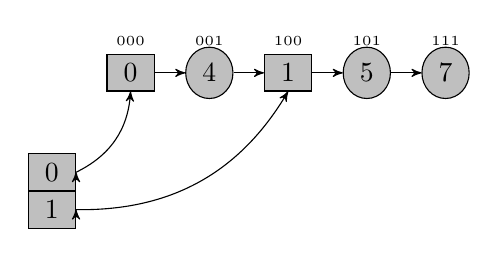
\begin{tikzpicture}[>=stealth',node distance=1cm]
\node[draw=black!100,fill=black!25,rectangle split,rectangle split allocate boxes=2,
      rectangle split parts=2,anchor=north,
      minimum width=6mm] at (0,2) (next1) 
      {$0$ \nodepart{two} $1$ };
\node[above of=next1,node distance=1.5cm] (anchor) {};
\node[draw=black!100,fill=black!25,rectangle, minimum width=6mm,right of=anchor] (0) {$0$};
\node[above of=0,node distance=4mm,font=\tiny] {$000$};
\node [right of=0,ellipse,draw=black!100,minimum width=6mm,fill=black!25] (4) {$4$} 
    edge[<-] (0);
\node[above of=4,node distance=4mm,font=\tiny] {$001$};
\node [right of=4,rectangle,draw=black!100,minimum width=6mm,fill=black!25] (1) {$1$} 
    edge[<-] (4);     
\node[above of=1,node distance=4mm,font=\tiny] {$100$};   
\node [right of=1,ellipse,draw=black!100,minimum width=6mm,fill=black!25] (5) {$5$} 
    edge[<-] (1);
\node[above of=5,node distance=4mm,font=\tiny] {$101$}; 
\node [right of=5,ellipse,draw=black!100,minimum width=6mm,fill=black!25] (7) {$7$} 
    edge[<-] (5);
\node[above of=7,node distance=4mm,font=\tiny] {$111$}; 
\draw[->,bend right] (next1.text east) edge (0.south) ;  
\draw[->,bend right] (next1.two east) edge (1.south);    
\end{tikzpicture}
\end{center}
\caption{Layout of the split-ordered hash table}
\label{Layout2}
\end{figure}

\begin{figure}
\begin{center}
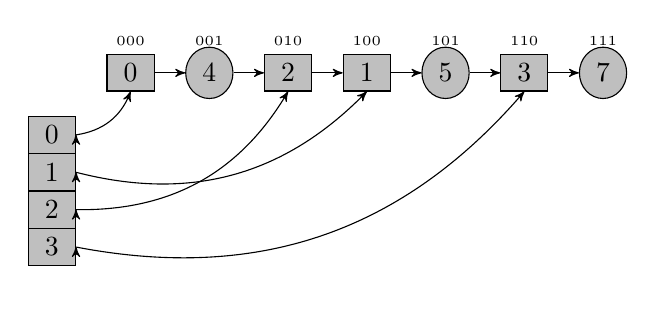
\begin{tikzpicture}[>=stealth',node distance=1cm]
\node[draw=black!100,fill=black!25,rectangle split,rectangle split allocate boxes=4,
      rectangle split parts=4,anchor=north,
      minimum width=6mm] at (0,2) (next1) 
      {$0$ \nodepart{two} $1$ \nodepart{three} $2$
      \nodepart{four}$3$};
\node[above of=next1,node distance=1.5cm] (anchor) {};
\node[draw=black!100,fill=black!25,rectangle, minimum width=6mm,right of=anchor] (0) {$0$};
\node[above of=0,node distance=4mm,font=\tiny] {$000$};
\node [right of=0,ellipse,draw=black!100,minimum width=6mm,fill=black!25] (4) {$4$} 
    edge[<-] (0);
\node[above of=4,node distance=4mm,font=\tiny] {$001$};
\node [right of=4,rectangle,draw=black!100,minimum width=6mm,fill=black!25] (2) {$2$} 
    edge[<-] (4);     
\node[above of=2,node distance=4mm,font=\tiny] {$010$};
\node [right of=2,rectangle,draw=black!100,minimum width=6mm,fill=black!25] (1) {$1$} 
    edge[<-] (2);     
\node[above of=1,node distance=4mm,font=\tiny] {$100$};   
\node [right of=1,ellipse,draw=black!100,minimum width=6mm,fill=black!25] (5) {$5$} 
    edge[<-] (1);
\node[above of=5,node distance=4mm,font=\tiny] {$101$}; 
\node [right of=5,rectangle,draw=black!100,minimum width=6mm,fill=black!25] (3) {$3$} 
    edge[<-] (5);
\node[above of=3,node distance=4mm,font=\tiny] {$110$}; 
\node [right of=3,ellipse,draw=black!100,minimum width=6mm,fill=black!25] (7) {$7$} 
    edge[<-] (3);
\node[above of=7,node distance=4mm,font=\tiny] {$111$}; 
\draw[->,bend right] (next1.text east) edge (0.south) ;  
\draw[->,bend right] (next1.two east) edge (1.south); 
\draw[->,bend right] (next1.three east) edge (2.south); 
\draw[->,bend right] (next1.four east) edge (3.south);             
\end{tikzpicture}
\end{center}
\caption{Layout of the split-ordered hash table}
\label{Layout3}
\end{figure}
 
Accessing an element in the hash table is straightforward; one merely needs to consider the top $n$ bits of the reverse bit order representation of the key (where $n$ is the current size of the table, in bits).  For example, to search for 7 in a 1-bit table, we would first access bucket 1 and then follow the {\em next} pointers until either we find our target, the next bucket, or the end of the list.  In the 2-bit table (Fig.~\ref{Layout3}), we would instead start our search at bucket 3.

The skiplist is a probabalistic data structure consisting of a hierarchy of ``levels''.  The lowest level of the skiplist consists of a linked list containing every element in the set.  Each higher level consists of a list that is a subset of the list immediately below it.  In order to locate a given element, a thread starts at the highest list and locates the (half-open) $(pred,curr]$ window containing the element in question.  The thread stores this window for the current level, then drops down to the next-lowest list and, starting at $pred$, searches for the window associated with that level.  This continues until the thread finds the $(pred,curr]$ window at the lowest level of the list.

In this skiplist, each element is inserted at a random level; each thread will  

\begin{figure}
\begin{center}
\begin{tikzpicture}[>=stealth',node distance=12mm]
\node[draw=black!100,fill=black!25,rectangle split,rectangle split allocate boxes=4,
      rectangle split parts=4,
      minimum width=6mm] (node0) 
      { };
      \node[below of=node0, node distance=8mm, font=\small,anchor=north] (0) {$-\infty$}; 
\node[draw=black!100,fill=black!25,rectangle split,
      rectangle split parts=1, anchor=south, minimum width=6mm,
      right= of node0.south, anchor=south] (node1) {}
      edge[<-] (node0.four south |- node0.four east);   
      \node[right of=0, font=\small] (1) {$5$};
\node[draw=black!100,fill=black!25,rectangle split,
      rectangle split parts=2, anchor=south, minimum width=6mm,
      right= of node1.south, anchor=south] (node2) {};
\draw (B1''.two split south) -- (B1''.north east);
      edge[<-] (node1.center);   
      \node[right of=1, font=\small] (2) {$7$};
\end{tikzpicture}
\end{center}
\caption{Layout of a skiplist}
\end{figure}
\section{Conclusions and Future Work}\label{Section:Conclusions}

Braginsky and Petrank described a means to reorganize a linked list to improve locality of memory
access; in this paper we have improved upon their algorithms.  By storing multiple keys in a node
and skipping irrelevant nodes, we can improve performance within a constant factor over traditional
linked lists.  Storing the entries
in an unsorted array allows us to sequentially scan these entries, a task which compilers can
aggressively and effectively optimize.  Our results are extremely encouraging and suggest that
further research should be done in this area.

We envision three different ideas for further research.  One possible improvement involves the
use of a {\em group mutual exclusion} object to control access to a node
\cite{Joung:GroupME}; this would permit
multiple {\em insert} or multiple {\em remove} operations to operate on the same node concurrently.
Second, we can develop a lock-free implementation of this object.  We would expect either technique
to provide an incremental performance improvement over what we have presented. 

Additionally, we would like to explore the potential of unrolling other, more complex, data
structures.  We imagine that certain implementations of concurrent hash tables (such as those presented by Shalev and Shavit \cite{Shalev:SplitOrder}) and concurrent skiplists (such as those by Herlihy\cite{Herlihy:Skiplist1} and Fraser\cite{FraserPhD}) would be amenable to this technique.
%\bibliographystyle{abbrv}
\bibliographystyle{splncs}
\bibliography{platz}

\end{document}